\chapter{État des lieux démographique}
\paragraph{}Les médias et les politiques nous rabâchent sans cesse que la population vieillit et que le système de pension n’est plus tenable. Mais qu’en est-il vraiment de la situation en Europe ?  Dans un premier temps, nous allons analyser la démographie actuelle dans l’Union européenne, ainsi que les projections existantes.

\paragraph{}Tout d'abord, quand on parle de vieillissement de la population, de quoi parle-t-on ? D’après l’encyclopédie Larousse~\citep{larousse}: 
\begin{quotation}
\textit{Le « vieillissement démographique » ou « vieillissement d'une population » désigne une modification progressive de la structure par âge de cette population. L'augmentation de la proportion des personnes âgées (60 ans et plus) s'accompagne d'une diminution, d'abord de la proportion des enfants (moins de 15 ans), puis de la proportion des personnes en âge de travailler (de 15 à 59 ans).}
\end{quotation}

\paragraph{}On retrouve une définition similaire ici~\citep{étudiant}.
\begin{quotation}
\textit{Le vieillissement désigne l’augmentation du poids des personnes âgées dans l’ensemble de la population.}
\end{quotation}

\paragraph{}Se doter d’une définition constitue une première étape importante mais il faut aussi être capable de mesurer ce vieillissement. Quels en sont les indicateurs ? Jacques Dupâquier ~\citep[pp.10-11]{dupaquier} en propose sept: 
\begin{enumerate}
  \item \textbf{L’effectif absolu de la population}. Il suffit de compter la population plus âgée qu’une limite définie: 60 ou 65 ans par exemple. Cette mesure isolée ne donne aucune indication par rapport au vieillissement de la population si la croissance constatée est proportionelle à la croissance globale de la population.
  \item \textbf{La proportion de la population âgée dans la population totale}.Il faut également définir un seuil, 60 ou 65 ans, mais cette mesure est très proche de la définition donnée plus haut. 
  \item \textbf{L'âge moyen de la population} et \textbf{l’âge médian de la population}. Ces mesures sont très simples et ne nécessitent pas de paramétrage. Une augmentation de ces chiffres fait effectivement le constat d’un vieillissement de la population, mais dans une perspective économique, cela ne donne pas assez d’informations. 
  \item \textbf{L’indice de vieillissement}, c’est-à-dire, le nombre de personnes âgées sur le nombre de jeunes. Il faut définir ici deux limites supérieures: la limite pour les jeunes est habituellement 15 ans et la limite pour les vieux est habituellement 60 ou 65 ans.
  \item \textbf{L’indice de sénescence}. Ici, il faut d’abord définir la limite entre les personnes âgées et celles non âgées; ensuite, définir une seconde limite pour les personnes très âgées (par exemple 75 ans); enfin, calculer le rapport personnes très âgées / total des personnes âgées. Cet indice ne permet pas de mesurer le vieillissement en tant que tel, mais il permet d'en connaître la nature.
  \item \textbf{L’indice de dépendance}. Cet indice consiste à calculer le rapport entre les personnes dépendantes et les personnes dont elles dépendent. Typiquement, les catégories des jeunes (-15 ans) et des personnes âgées (+65 ans) divisées par la catégorie intermédiaire (15 - 64 ans). Il peut se calculer en tenant seulement compte des personnes âgées. Cette mesure est très intéressante d’un point de vue économique. 
\end{enumerate}
\paragraph{} De ces sept mesures, nous en retiendrons principalement deux : la proportion de la population âgée dans la population totale, pour mesurer l’ampleur du phénomène, et l’indice de dépendance, qui permettra de mesurer certains aspects de l’impact du vieillissement. Dans un premier temps, nous utiliserons surtout la deuxième. Cependant, comme nous l’avons expliqué plus haut, pour pouvoir calculer cet indice, il faut choisir une limite arbitraire entre les personnes âgées et les autres. Dans ce document, nous nous intéresserons surtout aux aspects économiques du vieillissement de la population. Il serait donc intéressant de définir la tranche de personnes âgées comme les personnes qui ne font plus partie de la population active en raison de leur âge. Malheureusement, avec des régimes de retraite différents dans chaque pays~\citep{age_retraite}, et la notion de prépension, il n’est pas facile de définir une limite bien précise. Nous avons décidé de mettre la limite à 65 ans car cela correspond à l’âge de départ à la retraite le plus répandu et, surtout, parce que les données statistiques sont plus faciles à trouver pour cette limite. 

\section{Démographie de l'Europe}
\paragraph{}Maintenant que nous avons clarifié le concept de vieillissement, observons les chiffres de l’Europe. Dans un premier temps, nous avons compilé les données venant d'Eurostat~\citep{eurostat_pop}. Nous avons pris le nombre d’habitants de 25 pays de l’Union européenne, c’est-à-dire de tous les pays, à l’exception de Malte, Chypre et la Croatie. Pour ces pays, d'une part, les données manquaient et, d'autre part, leur population ne représentant qu'une infime proportion de la population européenne, nous supposons que les chiffres n’auraient pas influencé la tendance globale observée. Nous tirerons donc des conclusions pour toute l’Union européenne malgré le manque de données pour ces pays.

\paragraph{}Le graphique \ref{eu_demo} montre l’évolution de la population totale et celle de la population des personnes âgées de plus de 65 ans. On peut observer que la population totale est passée de 450 à 500 millions d’habitants entre 1975 et 2013, mais que la population de personnes âgées est passée de 55 millions à 91 millions. Elle a presque doublé en un peu moins de 40 ans. La population globale n’a pas augmenté dans les mêmes proportions. Le graphe \ref{pop_65} montre cet état de fait beaucoup plus clairement. Il montre l’évolution de la proportion de la population âgée de plus de 65 ans: elle est passée de 12\% à 18\% de la population globale en l’espace de 40 ans et surtout de 15,5\% à 18\% en l’espace de 13 ans: on voit que le phénomène s'accélère.  Et cela, alors que la proportion de personnes âgées de plus de 65 ans dans le monde n’est que de 12\%~\citep{ined}. Il est clair que la population de l’Europe est plus vieille que celle du reste du monde et que le vieillissement s’accentue d’année en année. 


\begin{figure}[h!]
    \begin{center}
        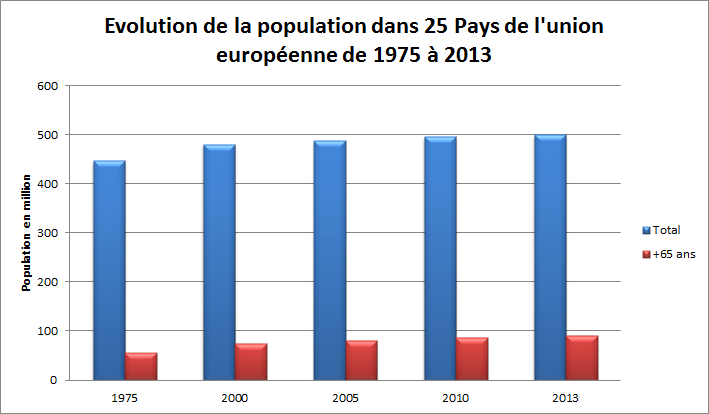
\includegraphics[scale=0.7]{document/pop_eu.png}
        \caption{Évolution de la population dans l'Union européenne de 1975 à 2015. Source: Eurostat~\citep{eurostat_pop}}
        \label{eu_demo}
    \end{center}
\end{figure}


\begin{figure}[h!]
    \begin{center}
        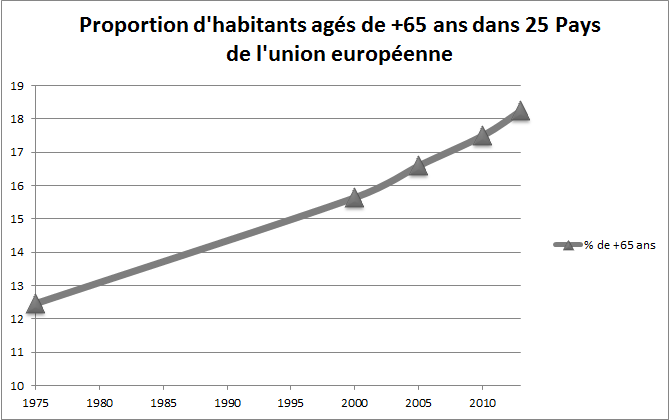
\includegraphics[scale=0.7]{document/pop_65.png}
        \caption{Évolution de la proportion de la population agée de plus de 65 ans dans l'Union européenne de 1975 à 2015. Source: Eurostat~\citep{eurostat_pop}}
        \label{pop_65}
    \end{center}
\end{figure}


\section{Disparité au sein de l'Union européenne}
\paragraph{}Derrière ces chiffres globaux se cachent parfois des réalités très différentes, comme nous allons l’observer pour la France et l’Allemagne. Si en l'an 2000, les deux pays avaient une proportion de 16\% de personnes âgées de plus de 65 ans, ce n’est plus du tout le cas en 2013, comme le montre le graphe \ref{fr-de_comparaison}. L’Allemagne a maintenant presque 21\% de sa population âgé de plus de 65 ans alors que la France est restée plus ou moins stable jusqu’en 2011 et n’atteint pas les 18\% de la moyenne européenne en 2013. La population continue à croître en France alors qu’elle diminue en Allemagne. Cette différence ne s’explique pas par l’immigration mais par des taux de natalité assez différents: 1,37 en Allemagne et 1,96 en France en 2007.~\citep[pp.5]{frde} La moyenne européenne était de 1,61 dans l’Europe des 28 en 2009. Les différences ne semblent pas importantes, mais le graphe \ref{fecondite}\footnote{Ce graphe a été construit en prenant 100 femmes pour la première génération et le nombre de femme des générations suivantes se calcule comme suit : $ NBF(X) = \frac{NBF(X-1) * Taux}{2}$} qui simule l’effet des différents taux de natalité sur la population, montre que pour 100 femmes à la première génération, l’effet cumulé des différents taux de fécondité est exponentiel. Avec un taux de fécondité de 1,38, il ne reste plus que 20 femmes lors de la 5ème génération alors qu’avec un taux de 1,6, il en reste le double. Avec un taux de fécondité supérieur à 2, la population augmente bien entendu.  
 
\begin{figure}[p]
    \begin{center}
        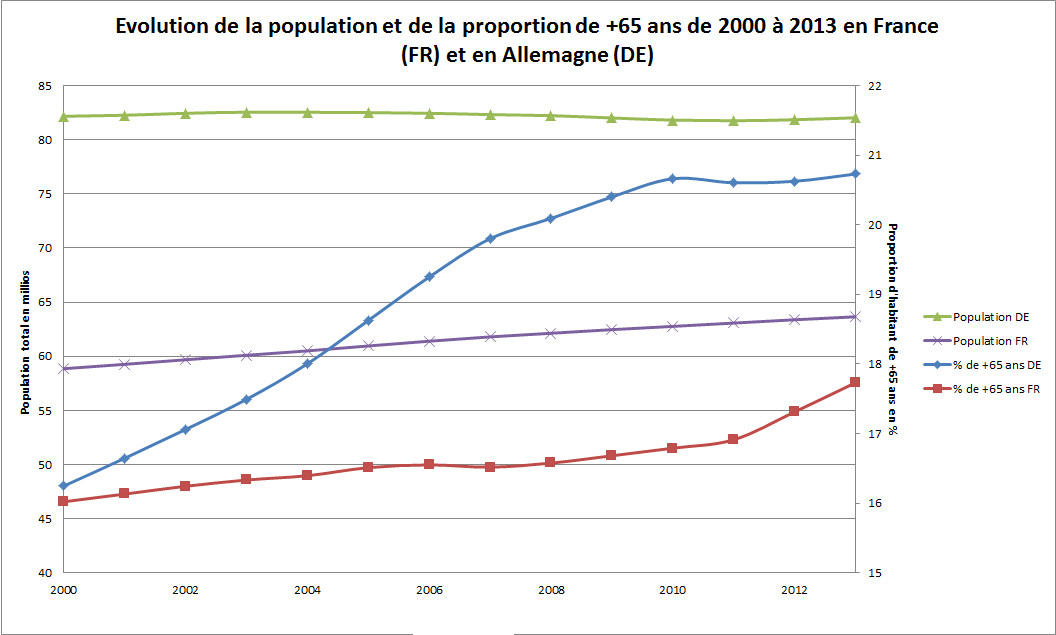
\includegraphics[scale=0.55]{document/fr-de_comparaison.png}
        \caption{Évolution de la population et de la proportion de la population agée de plus de 65 ans en France et en Allemagne de 2000 à 2015. Source: Eurostat~\citep{eurostat_pop}}
        \label{fr-de_comparaison}
    \end{center}
\end{figure}

\begin{figure}[p]
    \begin{center}
        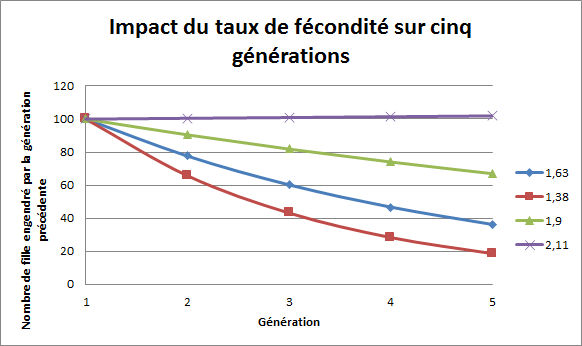
\includegraphics[scale=0.8]{document/fecondite.png}
        \caption{Simuluation de l'évolution du nombre de femmes avec différents taux de fécondité constants}
        \label{fecondite}
    \end{center}
\end{figure}

\paragraph{}Quel est le rapport entre le taux de fécondité et le vieillissement de la population ? Nous avons vu que chaque génération va en engendrer une autre, moins nombreuse, mais que les anciennes générations continuent à vivre un certain temps. Nous avons donc une pyramide des âges inversée qui devient plus petite à la base qu’au sommet et, automatiquement, la proportion des personnes plus âgées augmente. On peut déjà observer cela sur la pyramide des âges de l’Allemagne en 2008. Bien entendu, cet effet est atténué par l’immigration. Par contre, en France, il n’est pas visible: le bas de la pyramide a tendance à être droit.  En Allemagne, comme en France, on peut observer l’effet du “Baby Boom”\footnote{\textit{Le baby boom ou « pic de la natalité » est une augmentation importante du taux de natalité dans certains pays, juste après la fin de la Seconde Guerre mondiale. Les enfants nés durant cette période sont parfois appelés des « baby boomers » (voir simplement, au Canada, des « boomers »). Cette période s'étend de 1945 à 1975.}~\citep{baby-boom}} sur les tranches d'âge situées entre 35 et 60 ans, car elles sont significativement plus importantes. On peut observer également que cet effet a duré plus longtemps en France qu'en Allemagne.

\paragraph{}Le cas de l’Allemagne est symptômatique. Beaucoup de pays européens présentent une courbe similaire à celle de l’Allemagne en 2010 (figure \ref{pyramide-Allemagne-France}), avec une base moins resserrée, car l’Allemagne est l'un des pays ayant le plus faible taux de natalité. La France, quant à elle, avec son taux supérieur à 2, constitue davantage une exception. C’est donc tout naturellement que la pyramide de l’Europe (Figure \ref{eu-2006}) présente une base plus étroite et que les tranches d'âge de personnes nées pendant le “Baby Boom” sont plus larges. 

\paragraph{}Après avoir fait le constat sur le passé et le présent, il est intéressant de se tourner vers l’avenir et de regarder du côté des projections démographiques. Les pyramides que nous venons d’observer n’augurent rien de bon. La mise à la retraire des Baby Boomers vient à peine de commencer et ne s’achèvera que dans 25-30 ans. Il est intéressant de comprendre les causes de ce vieillissement pour mieux comprendre ce que le futur nous réserve. 

\begin{figure}[p]
    \begin{center}
        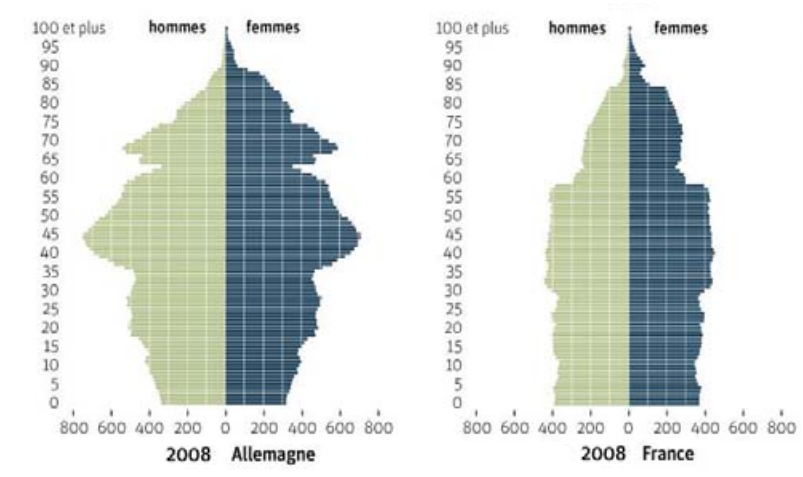
\includegraphics[scale=0.55]{document/pyramide-allemagne-france.png}
        \caption{Pyramide des âges de l'Allemagne à gauche et de la France à droite. Source: Sievert~\citep[pp.27]{frde}}
        \label{pyramide-allemagne-france}
    \end{center}
\end{figure}

\begin{figure}[p]
    \begin{center}
        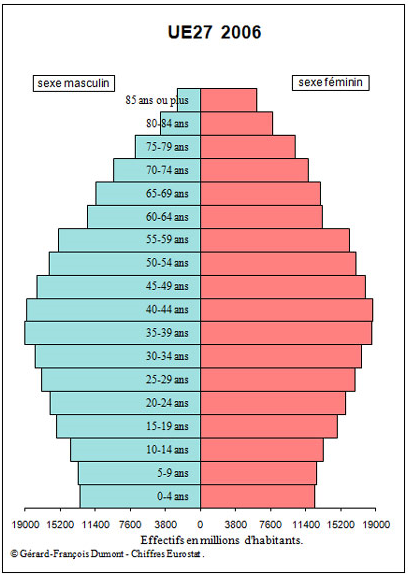
\includegraphics[scale=0.55]{document/eu-2006.png}
        \caption{Pyramide des âges de l'Union européenne en 2006 Source: Dumont~\citep[pp.3]{pyramide-eu}}
        \label{eu-2006}
    \end{center}
\end{figure}


\section{Facteurs explicatifs du vieillissement démographique}
\paragraph{}Maintenant que nous avons constaté le vieillissement effectif de la population, il est faut s'interroger sur ses causes. L’article de Francois Héran~\citep[pp.1]{heran} identifie quatre causes. La première, dite “vieillissement par le bas”, peut s'observer via son effet de rétrécissement de la base de la pyramide. Cet effet est dû à une fécondité durablement sous le seuil de remplacement\footnote{\textit{Le seuil de renouvellement (ou de remplacement) des générations, c'est-à-dire le nombre moyen d'enfants par femme nécessaire pour que chaque génération en engendre une suivante de même effectif, est au minimum de 2,05 enfants par femme, soit 205 enfants pour 100 femmes, parce que pour 105 garçons, il naît 100 filles. Les seuils réels sont supérieurs à ce minimum en raison de la mortalité entre la naissance et l'âge de procréation.}~\citep{renouvellement}
}, actuellement de 2,07 en Europe. Le graphe \ref{fertilite_eu} montre le taux de fertilité de ces 15 dernières années dans l’Europe des 28. La tendance est claire: le taux de fertilité est bien en-dessous du taux de remplacement et il n’est pas prêt à remonter. Du fait de la diminution du nombre de jeunes, la proportion de personnes âgées augmente de facto.  

\paragraph{}Le second effet est ce qu’Héran appelle~\citep[pp.1]{heran}, le “vieillisement par le haut”, c’est-à-dire, l’ajout d’étages au somment de la pyramide des âges, dû à l’augmentation de l’espérance de vie.  Les personnes de plus de 65 ans vieillissent au lieu de mourir. Cette progression de l’espérance de vie a dépassé les projections. Chaque année, un gain de deux à trois mois est observé. Ce facteur est vu comme inévitable car personne ne peut mettre en place une politique qui vise à réduire la progression de l’espérance de vie.

\paragraph{}Le troisième facteur est lié à une forte variation de la natalité dans le passé~\citep[pp.2]{heran} : Le Baby Boom, suivi d'un retour à la “normale”. Ces trente années de fertilité exceptionnelle ont eu comme effet premier de rajeunir la population; ensuite de grossir les rangs de la population active pendant des dizaines d’années; mais, maintenant, il vient participer à l’accélération du vieillissement pour finalement faire monter le taux de mortalité. Si l'on observe l’évolution d’une pyramide des âges dans un pays tel que la Belgique, on peut voir clairement une vague se former dès les années 50 et se déplacer. Elle se situe actuellement autour de la tranche des personnes de 55 ans~\citep{pyramide-be}. Ce facteur est, lui aussi, inévitable, car aucune politique démographique ne peut l’influencer, c’est une conséquence des politiques passées.

\paragraph{}Le dernier facteur~\citep[pp.3]{heran}, plus anecdotique, est l’émigration sélective des jeunes. Ce phénomène peut s’observer en Albanie par exemple.

\begin{figure}[h!]
    \begin{center}
        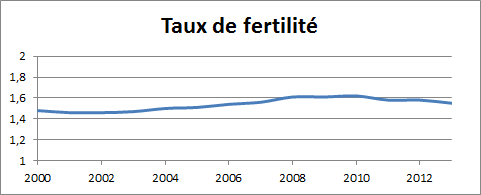
\includegraphics[scale=1]{document/fertilite_eu.png}
        \caption{Variation du taux de fertilité pour l'Europe des 28 de 2000 à 2013.  Source: Eurostat~\citep{eurostat_fecondite}}
        \label{fertilite_eu}
    \end{center}
\end{figure}

\section{Projection démographique}
\paragraph{}Deux projections sont facilement disponibles pour l’Europe: celle de l’ONU~\citep{onu} et celle d’Eurostat~\citep{eurostat_europop13}. Les données d’Eurostat concernant plus spécifiquement l’Union européenne, le sujet de notre étude, nous nous focaliserons essentiellement sur celles-ci.  

\subsection{Les hypothèses des projections d’Eurostat}
\paragraph{}Les projections sont construites sur base d’une année de référence, ici 2013 pour EUROPOP2013~\citep{eurostat_europop13}, selon la formule suivante:
$$ Pop_{1.1.n+1} = Pop_{1.1.n} + naissances_{n} - deces_{n} + solde migratoire_{n} $$ ~\citep[pp.3]{INSEE}
où $Pop_{1.1.n}$ est la population au premier janvier de l'année n et $Pop_{1.1.n+1}$ est la population au premier janvier de l'année suivante. Cette formule, assez simple, dissimule des éléments complexes: les naissances sont basées sur le nombre de femmes à l’année n, sur leurs âges et sur le taux de fécondité. Les décès sont basés sur un quotiant de mortalité, lui-même différent à chaque âge et dépendant de l’espérance de vie, auquel il faut ajouter la mortalité des nouveau-nés~\citep[pp.4]{INSEE}. Bien sûr, le solde migratoire est basé sur l’immigration et l’émigration à l’intérieur du territoire qu’on étudie. Le rapport “The 2015 Ageing Report” décrit en détails toutes les hypothèses échafaudées sur ces paramètres~\citep[pp.8-14]{ageing_methodo}. Dans les grandes lignes, la projection EUROPOP2013 utilise une approche convergeante: tous les paramètres convergent et se stabilisent sur une très longue période de temps. Un point de convergence éloigné permet de tenir compte des tendances actuelles, mais aussi de partir de l’hypothèse d’une convergence des paramètres sur le long terme. La projection se base sur un taux de fertilité en augmentation, qui convergerait vers 1.76 en 2060~\citep[pp.9]{ageing_methodo}. Elle envisage que l’espérance de vie augmente encore de 7,2 ans pour les hommes (84,7 and en 2060) et des 6 ans pour les femmes, jusqu’en 2060 (89 ans en 2060)~\citep[pp.11]{ageing_methodo}. Le taux de migration est certainement la donnée la plus variable: la projection estime à 55 millions le solde migratoire cumulé sur les années de la projection~\citep[pp.14]{ageing_methodo}. Nous ne détaillerons pas ici tous les détails des hypothèses, ni les calculs qu’ils impliquent, car nous serions bien au-delà du cadre de ce document. 

\paragraph{}Eurostat fournit cinq scénarios: un scénario principal, un scénario sans migration, une variante de migration basse (48 millions de solde migratoire sur la période jusqu’en 2060),  un scénario avec une espérance de vie haute (en 2060, 86,1 ans pour les hommes et 90,6 ans pour les femmes en 2060) et une hypothèse de fécondité basse (qui converge vers 1,39 en 2060). La table \ref{projection_scenario} présente les résultats de chaque scénario pour 2060 et 2080.

\begin{table}
  \caption{Projection de la population totale dans l'Europe des 28 selon les différents scénarios d'Eurostat EUROPOP13 source: Eurostat~\citep{eurostat_europop13}}
  \label{projection_scenario}

  \begin{center}
    \begin{tabular}{lcc}
       & Population en 2060 & Population en 2080\\
      Scénario principal & 522.945.539 & 520.035.469\\
      Sans migration & 442.752.273 & 399.215.880 \\
      Migration basse & 515.880.322 & 506.906.909 \\
      Espérance de vie haute & 528.301.525 & 533.900.985 \\
      Fécondité basse & 516.144.576 & 497.707.180 \\
    \end{tabular}
  \end{center}
\end{table}

\paragraph{}Mis à part dans le scénario d’une espérance de vie haute, la population entre 2060 et 2080 diminue. Le scénario sans migration est le plus distant du scénario principal et amène une diminution de 43 millions d’habitants en 20 ans. C’est celui qui fait l’hypothèse la plus extrême: il met en avant le rôle majeur de l’immigration dans le maintien de la population européenne.


\subsection{Analyse du scénario principal des projections Eurostat}
\paragraph{}Regardons maintenant plus en détails le scénario principal. Nous allons reprendre les mêmes indicateurs que dans les sections précédentes pour quantifier le vieillissement de la population. 

\paragraph{}Le graphe \ref{proj_pop} montre l’évolution de la population jusqu’en 2080 ainsi que l’évolution de l’âge moyen de la population. La population augmente jusqu’en 2050 et l’âge moyen de la population augmente jusqu’en 2040. On peut observer une nette corrélation entre la population et l’âge moyen de la population, ce qui veut dire que l’augmentation de la population est due à l’ajout d’étages à la pyramide des âges. Le processus de mortalité des personnes nées pendant le Baby Boom commence en 2040 pour s’achever en 2070. Ce n’est qu’en 2070 que l’Union européenne cessera de subir les conséquences du taux de fertilité du Baby Boom. 


\begin{figure}[h!]
    \begin{center}
        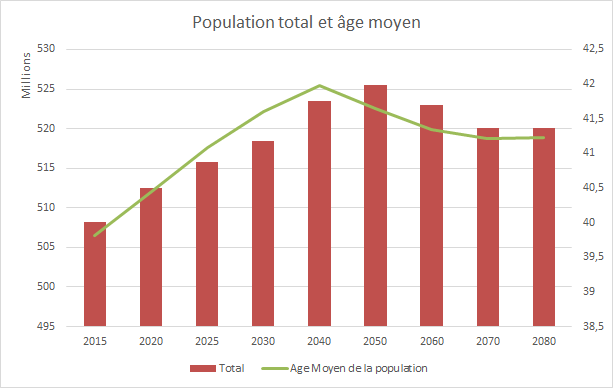
\includegraphics[scale=0.7]{document/proj_pop.png}
        \caption{Projection de la population totale et de l'âge moyen de cette population de 2015 à 2080 dans l'Europe des 28. Source: Eurostat~\citep{eurostat_europop13}}
        \label{proj_pop}
    \end{center}
\end{figure}

\paragraph{}Le graphe \ref{proj_prop} présente l’évolution de la proportion de personnes âgées. La courbe suit la tendance observée dans le graphe précédent. La proportion passera de 15\% à 20\% en 2040 pour se stabiliser en 2070 autour de 18\%. Ce graphe montre que si le vieillissement de la population est déjà un problème maintenant, il sera supérieur en 2040 (33\%). Il faudra donc trouver des solutions à long terme.

\begin{figure}[h!]
    \begin{center}
        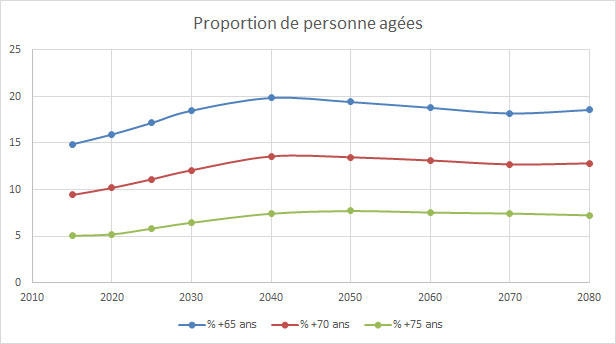
\includegraphics[scale=0.7]{document/proj_prop.png}
        \caption{Projection de l'évolution de la proportion de personnes agées dans la population dans l'Europe des 28 de 2015 à 2080. Source: Eurostat~\citep{eurostat_europop13}}
        \label{proj_prop}
    \end{center}
\end{figure}

\paragraph{}Le graphe \ref{dependance} permet de prendre pleinement la mesure du problème. Il mesure le degré de dépendance, c'est à dire le nombre de personnes qu’une personne active aura à charge. Bien entendu, ce graphe ne tient pas compte des personnes non actives en raison de chômage, de maladie ou de handicap. Le degré de dépendance est de 60\% en 2050, pourcentage causé principalement par les personnes âgées\footnote{ Elles pèsent pour 56\% dans l’indice : 34/60}. La courbe de dépendance totale est essentiellement corrélée à la courbe de dépendance des personnes âgées car le nombre d’enfants âgés de moins de 15 ans reste stable. 



\begin{figure}[h!]
    \begin{center}
        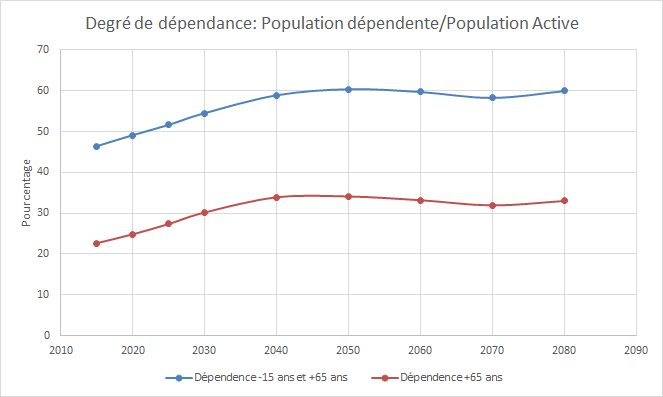
\includegraphics[scale=0.6]{document/dependance.png}
        \caption{Projection de l'évolution du degré de dépendance dans la population dans l'Europe des 28 de 2015 à 2080. Source: Eurostat~\citep{eurostat_europop13}}
        \label{dependance}
    \end{center}
\end{figure}

%TODO
\paragraph{}Dans le prochain chapitre, nous allons analyser les conséquences économiques et sociales de ce vieillissement durable pour l’Union européenne.
